\documentclass{article}
\usepackage{geometry}
\usepackage{tikz}
\usetikzlibrary{automata, positioning, arrows}

\tikzset{
    %Define standard arrow tip
    >=stealth',
    %Define style for boxes
    squ/.style={
           rectangle,
           rounded corners,
           draw=black, very thick,
           minimum height=2em,
           text centered},
  %different type of node
    ELt/.style={
	rectangle,
	draw=black, very thick,
	minimum height=3em,
	minimum width=10em,
	fill=blue,
	opacity=0.15,
	text centered,
	text opacity=1},
    % Define arrow style
    pil/.style={
           ->,
           thick,
           shorten <=2pt,
           shorten >=2pt,}
}


\begin{document}
\flushleft
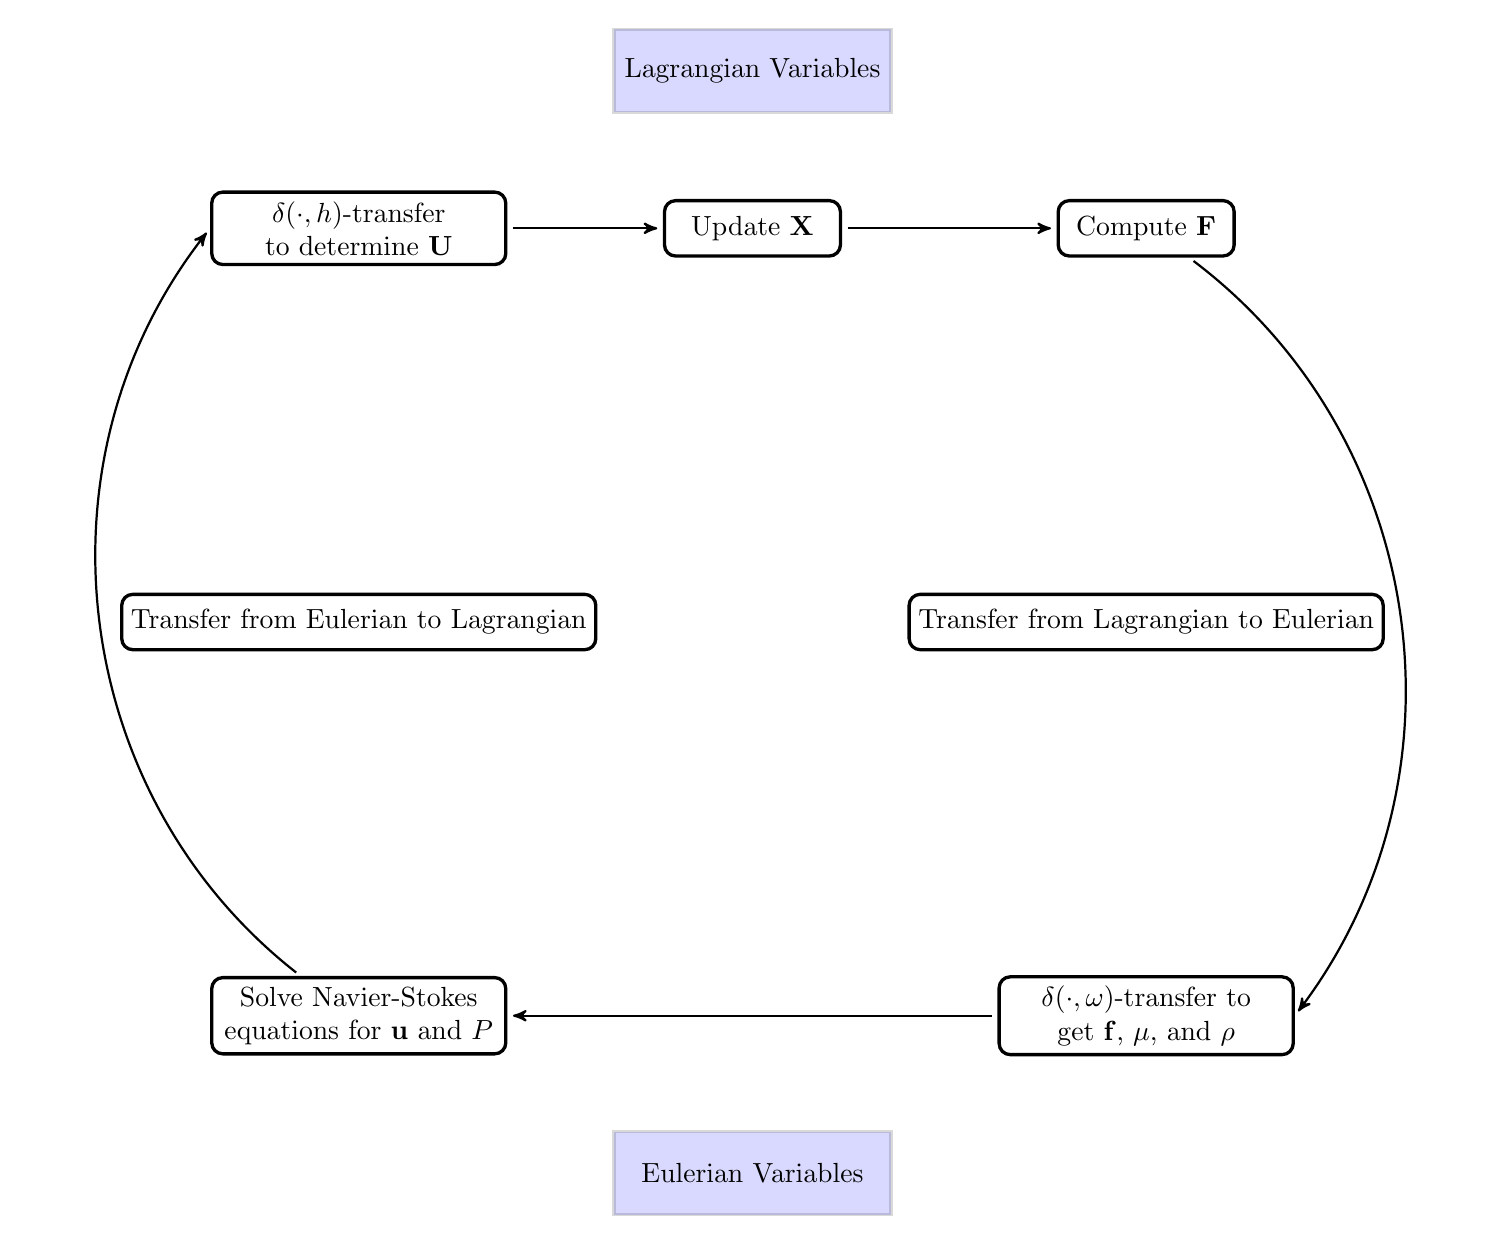
\begin{tikzpicture}

%\pgftext { \includegraphics[width=1\textwidth]{biofilmimage.png}} at (0pt, 0pt);

\node[squ] (A) at (0,0)   [rectangle ,text width =3.5cm, draw]{Solve Navier-Stokes equations for $\mathbf{u}$ and $P$};
\node[squ] (B) at (0,10) [ rectangle,  text width =3.5cm, draw]{$\delta(\cdot, h)$-transfer to determine $\mathbf{U}$};
\node[squ](C) at (5,10) [ rectangle, text width=2cm, draw] {Update $\mathbf{X}$ };
\node[squ] (D) at (10,10) [rectangle, text width =2cm, draw] {Compute $\mathbf{F}$};
\node[squ] (E) at(10,0) [rectangle, text width=3.5cm, draw]{$\delta(\cdot, \omega)$-transfer to get $\mathbf{f}$, $\mu$, and $\rho$};
\node[squ] (EL) at (0,5) {Transfer from Eulerian to Lagrangian};
\node[squ] (LE) at (10,5){Transfer from Lagrangian to Eulerian};
\node[ELt] (Eul) at (5,-2){Eulerian Variables};
\node[ELt] (Lag) at (5,12){Lagrangian Variables};

\path
 (A)	edge[pil, bend left=45] (B.west)
(B)	edge[pil, bend left=0] (C.west)
(C)      edge[pil, bend left=0] (D.west)
(D)	edge[pil, bend left=45] (E.east)
(E)	edge[pil, bend left=0] (A.east);


\end{tikzpicture}

\end{document}